\begin{frame}
    \titlepage
\end{frame}

\begin{frame}
    \frametitle{Outline}
    \tableofcontents
\end{frame}

\section{Introduction}

\begin{frame}
    \frametitle{First-order phase transitions}
    \begin{columns}
    \begin{column}{0.5\textwidth}
        \begin{itemize}
            \item If there is a potential barrier between the local and global minima, the phase transition is of first order
            \item Standard Model Higgs transition is of second order, but various extensions convert it to first order
            \item Klein-Gordon equation with a friction term
            \begin{equation}
                \Box \phi - V_T'(\phi) = - \eta_T(\phi) u^\mu \partial_\mu \phi
            \end{equation}
            \textrightarrow \ Constant wall speed
        \end{itemize}
    \end{column}
    \begin{column}{0.5\textwidth}
        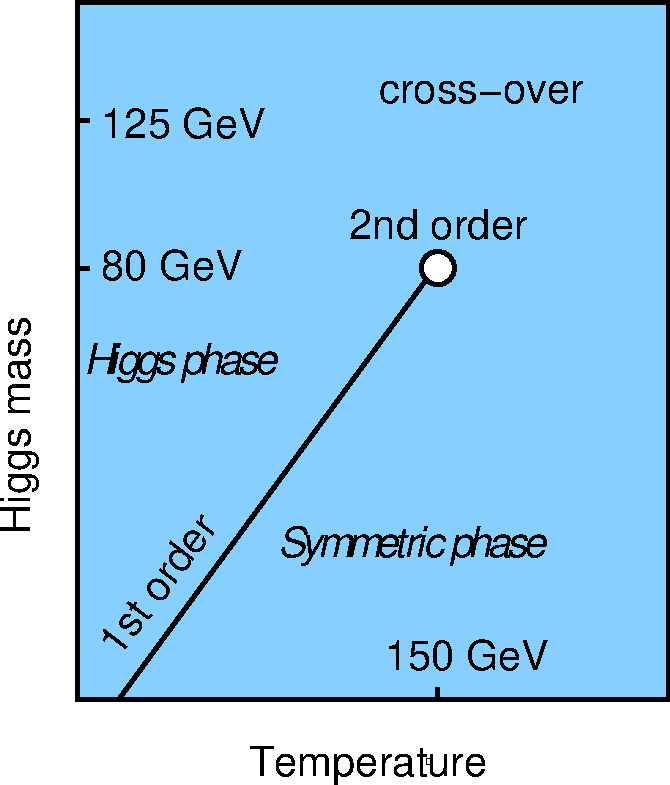
\includegraphics[width=0.45\textwidth]{../fig/smPhaseDiag2}%
        \hfill%
        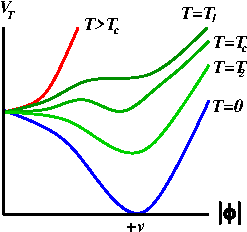
\includegraphics[width=0.45\textwidth]{../fig/ThermalHiggsPotential}
    \end{column}
    \end{columns}
\end{frame}

\begin{frame}
    \frametitle{Bubble nucleation}
    \begin{columns}
    \begin{column}{0.6\textwidth}
        \begin{itemize}
            \item Spontaneous tunneling to the new phase \textrightarrow \ bubble nucleation and expansion
            \item Bubble expansion is governed by relativistic hydrodynamics
            \item "Trying to determine the properties of a fluid in a water kettle based on the sound of boiling"
            \begin{itemize}
                \item Listening to the sound indirectly through GWs
            \end{itemize}
            \item Energy-momentum conservation gives rise to
            \begin{itemize}
                \item Wave equation
                \item Bubble wall junction conditions
                \item Continuity equations, aka. hydrodynamic equations
            \end{itemize}
        \end{itemize}
    \end{column}
    \begin{column}{0.4\textwidth}
        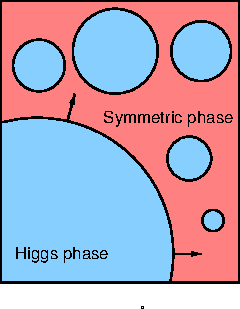
\includegraphics[width=0.33\textwidth]{../fig/HiggsBubble1}%
        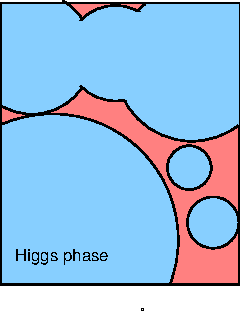
\includegraphics[width=0.33\textwidth]{../fig/HiggsBubble2}%
        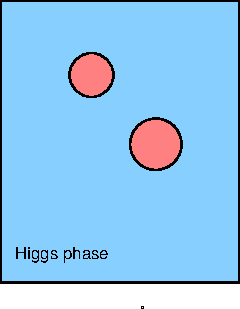
\includegraphics[width=0.33\textwidth]{../fig/HiggsBubble3}
    \end{column}
    \end{columns}
\end{frame}

\section{Phase transition bubble hydrodynamics}

\begin{frame}
    \frametitle{Dimensionality of the problem}
    \begin{itemize}
        \item Self-similarity
        \begin{itemize}
            \item Friction results in a constant wall speed $v_\text{wall}$
            \item As the bubble expands, its shape stays the same
            \item \textrightarrow \ Time-independent solution
        \end{itemize}
        \item Spherical symmetry
        \item 3+1 dimensional problem reduces to time-independent 1D
    \end{itemize}
\end{frame}

\iffalse
\begin{frame}
    \frametitle{Energy-momentum tensor}
    \begin{itemize}
        \item In Minkowski space and Cartesian coordinates
        \begin{equation}
        T_{\mu \nu} =
        \begin{bmatrix}
        e & -q_1 & -q_2 & -q_3 \\
        -q_1 & p + \Pi_{11} & \Pi_{12} & \Pi_{13} \\
        -q_2 & \Pi_{12} & p + \Pi_{22} & \Pi_{23} \\
        -q_3 & \Pi_{13} & \Pi_{23} & p + \Pi_{33}
        \end{bmatrix},
        \label{eq:ep_tensor_general_matrix}
        \end{equation}
        \item Ideal fluid: in the rest frame of the fluid $T^{0j} = 0, \quad i \neq j: \ T^{ij} = 0$
        \begin{equation}
        T_{\mu \nu} =
        \begin{bmatrix}
        e & 0 & 0 & 0 \\
        0 & p & 0 & 0 \\
        0 & 0 & p & 0 \\
        0 & 0 & 0 & p
        \end{bmatrix}
        \quad \quad
        T^{\mu \nu}_f = (e+p) u^\mu u^\nu + p g^{\mu \nu}
        \end{equation}
        \item Pressure $p = \frac{1}{3} T^i_i$
    \end{itemize}
\end{frame}
\fi

\begin{frame}
    \frametitle{Wave equation}
    \begin{itemize}
        \item Constant background space-time \textrightarrow \ energy-momentum conservation $\nabla_\mu T^{\mu\nu} = 0$
        \item Energy-momentum tensor of an ideal fluid
        \begin{equation}
            T^{\mu \nu}_f = (e+p) u^\mu u^\nu + p g^{\mu \nu}
        \end{equation}
        \item For a one-dimensional flow in Cartesian coordinates
        \begin{align}
            \partial_t \left[ (e+pv^2) \gamma^2 \right] + \partial_x \left[ (e+p) \gamma^2 v \right] &= 0,
            \label{eq:ep_conservation_1d_1} \\
            \partial_t \left[ (e+p) \gamma^2 v \right] + \partial_x \left[ (ev^2 + p) \gamma^2 \right] &= 0
            \label{eq:ep_conservation_1d_2}
        \end{align}
        \item First-order perturbation \textrightarrow \ wave equation with speed of sound
        \begin{equation}
            \partial_t^2 (\delta e) - \frac{\delta p}{\delta e} \partial_x^2(\delta e) = 0
            \quad \quad
            c_s^2 \equiv \frac{dp}{de} = \frac{dp/dT}{de/dT}
        \end{equation}
    \end{itemize}
\end{frame}

\begin{frame}
    \frametitle{Phase boundary}
    \begin{itemize}
        \item Energy-momentum conservation
        \begin{equation}
            \nabla_\mu T^{\mu\nu} = 0
            \quad \Rightarrow \quad
            \partial_z T^{zz} = \partial_z T^{z0} = 0
        \end{equation}
        \item Inserting ideal fluid $T^{\mu \nu}_f = (e+p) u^\mu u^\nu + p g^{\mu \nu}$ \textrightarrow \ Junction conditions
        \begin{align}
            w_- \tilde{\gamma}_-^2 \tilde{v}_- &= w_+ \tilde{\gamma}_+^2 \tilde{v}_+
            \label{eq:junction_condition_1} \\
            w_- \tilde{\gamma}_-^2 \tilde{v}_-^2 + p_- &= w_+ \tilde{\gamma}_+^2 \tilde{v}_+^2 + p_+
            \label{eq:junction_condition_2}
        \end{align}
        \item By defining new variables $\theta = \frac{1}{4}(e-3p), \quad \textcolor{red}{\alpha_+} \equiv \frac{4}{3} \frac{\theta_+(w_+) - \theta_-(w_-)}{w_+}, \quad r = \frac{w_+}{w_-}$
        \begin{align}
            \tilde{v}_+ &= \frac{1}{2(1+\textcolor{red}{\alpha_+})}\left[ \left(\frac{1}{3\tilde{v}_-}+\tilde{v}_-\right) \pm \sqrt{\left(\frac{1}{3\tilde{v}_-} - \tilde{v}_- \right)^2 + 4\textcolor{red}{\alpha_+}^2 + \frac{8}{3} \textcolor{red}{\alpha_+}} \right],
            \label{eq:v_tilde_plus}
            \\
            \tilde{v}_- &= \frac{1}{2} \left[ \left( (1+\textcolor{red}{\alpha_+})\tilde{v}_+ + \frac{1-3\alpha_+}{3\tilde{v}_+} \right) \pm \sqrt{\left((1+\textcolor{red}{\alpha_+})\tilde{v}_+ + \frac{1-3\textcolor{red}{\alpha_+}}{3\tilde{v}_+} \right)^2 - \frac{4}{3}} \right).
            \label{eq:v_tilde_minus}
        \end{align}
    \end{itemize}
\end{frame}

\begin{frame}
    \frametitle{Hydrodynamic equations}
    \begin{itemize}
        \item Energy-momentum conservation $\nabla_\mu T^{\mu\nu} = 0$
        \item Projection \textrightarrow \ hydrodynamic equations away from the phase boundary
        \begin{align}
            0 &= u_\mu \partial_\nu T^{\mu \nu} = -\partial_\mu (w u^\mu) + u^\mu \partial_\mu p, \\
            0 &= \bar{u}_\mu \partial_\nu T^{\mu \nu} = w \bar{u}^\nu u^\mu \partial_\mu u_\nu + \bar{u}^\mu \partial_\mu p.
        \end{align}
        \item Using self-similarity $\xi = \frac{r}{t}$
        \begin{align}
            \frac{d\xi}{d\tau} &= \xi \left[ (\xi - v)^2 - c_s^2 (1 - \xi v)^2 \right], \\
            \frac{dv}{d\tau} &= 2 v c_s^2 (1 - v^2) (1 - \xi v), \\
            \frac{dw}{d\tau} &= w \left( 1 + \frac{1}{c_s^2} \right) \gamma^2 \mu \frac{dv}{d\tau}.
        \end{align}
    \end{itemize}
\end{frame}

\begin{frame}
    \frametitle{Fluid shells}
    \begin{itemize}
        \item Three types of solutions, determined by
        \begin{itemize}
            \item Wall velocity $v_\text{wall}$
            \item Transition strength $\alpha_n$
            \item Speed of sound $c_s(T,\phi)$
        \end{itemize}
    \end{itemize}
    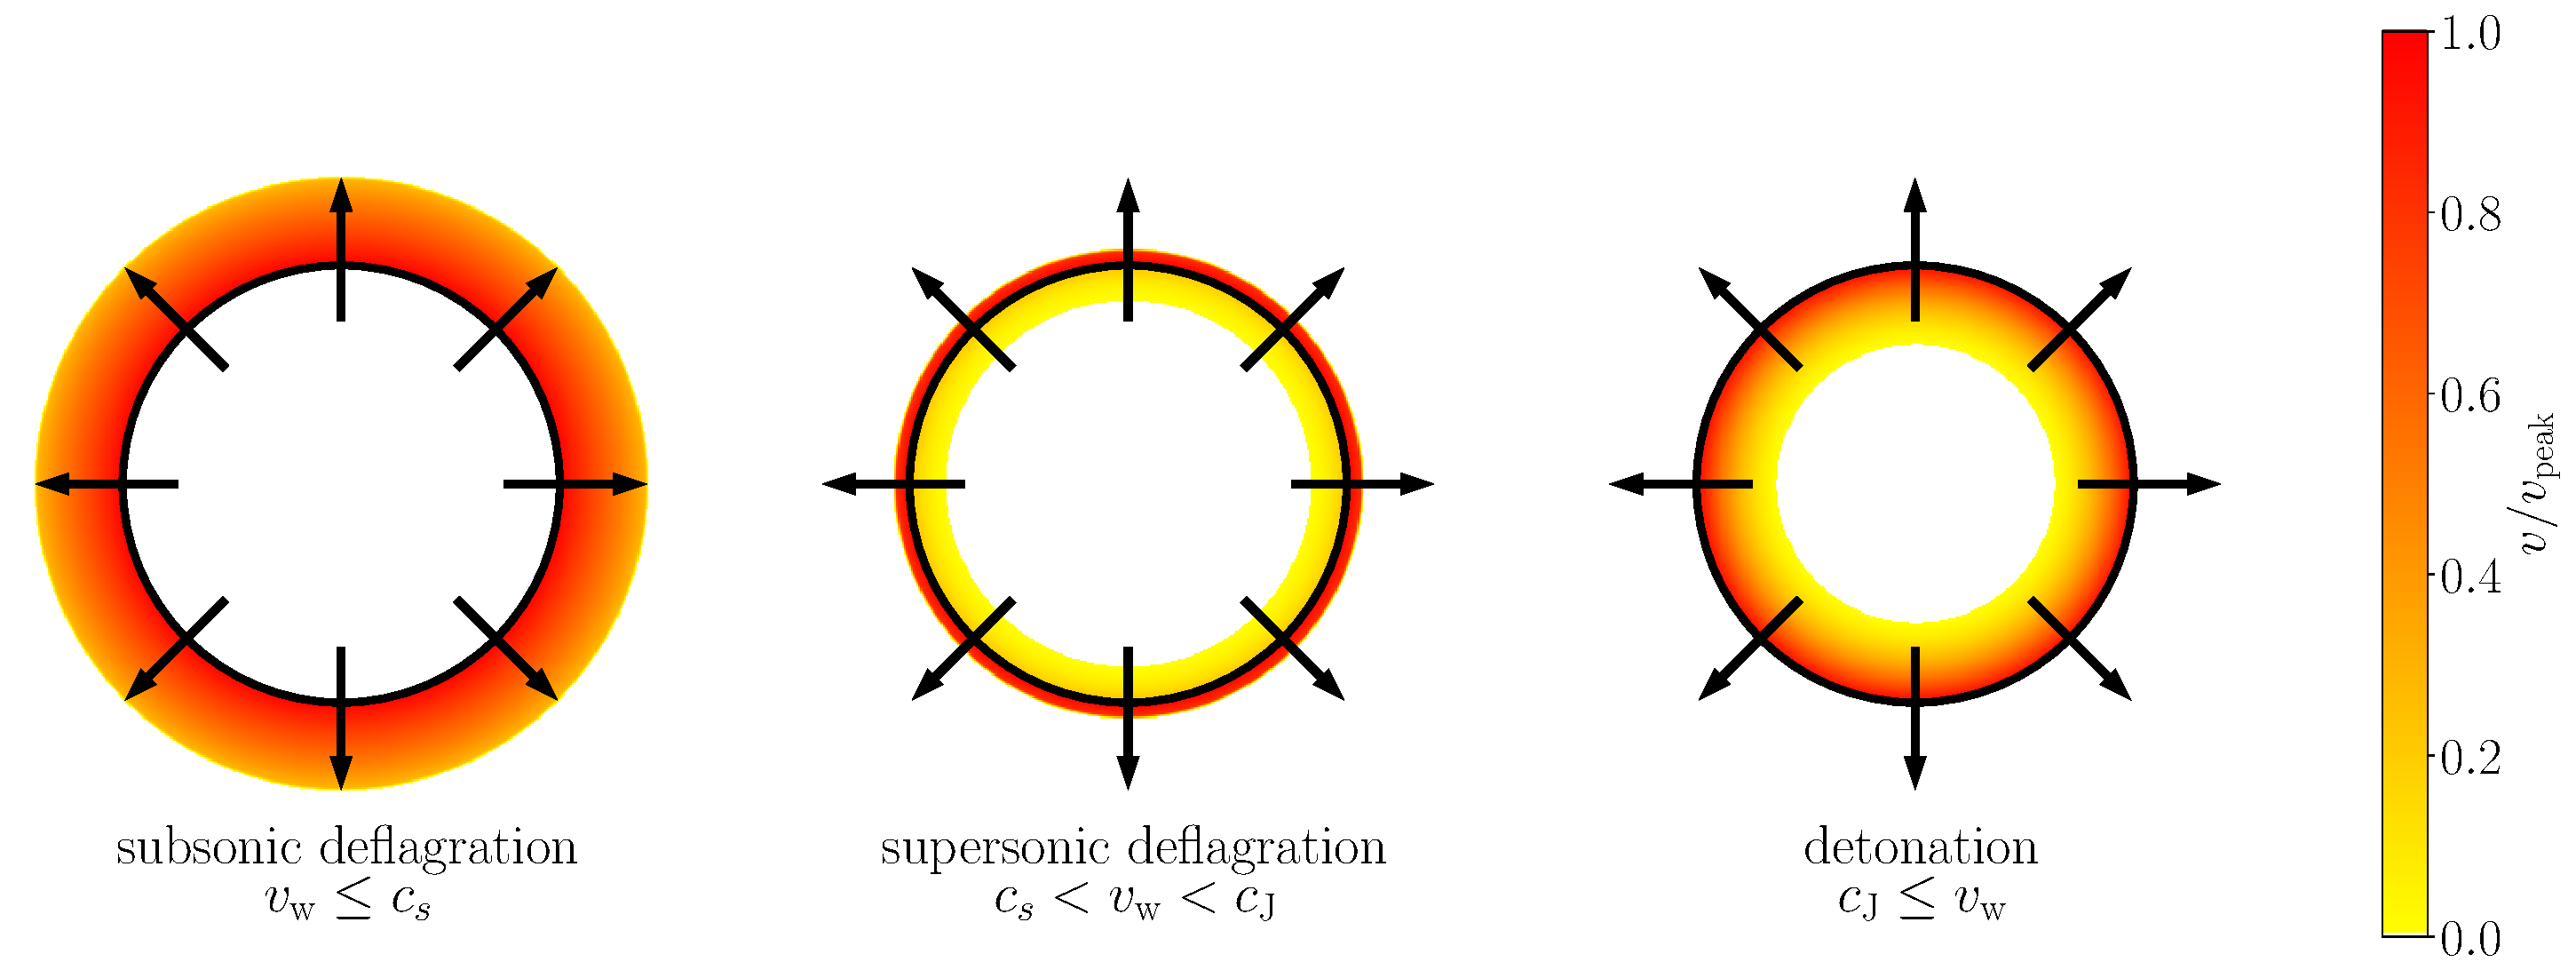
\includegraphics[width=0.8\textwidth]{../fig/all_circle.pdf} \\
    {\footnotesize Black = bubble wall / phase boundary}
\end{frame}

\section{Equations of state}

\begin{frame}
    \frametitle{General equation of state}
    \begin{itemize}
%        \item Energy-momentum tensor in momentum space
%        \begin{equation}
%            T^{\mu \nu}(x) = \int \frac{d^3 p}{(2 \pi)^3} \frac{p^\mu p^\nu}{p^0} f(\vec{p},x)
%        \end{equation}
%        \item Pressure
%        \begin{align}
%            p = \frac{1}{3} T^i_i
%            &= \frac{1}{3} \int \frac{d^3 p}{(2 \pi)^3} \frac{|\vec{p}|^2}{E} f(\vec{p},x) \quad \big| \ f(\vec{p}) = \frac{1}{e^\frac{E-\mu}{T} - 1}, \ \mu = 0\\
%            &= \frac{1}{6 \pi^2} \int_0^\infty \frac{p^3 dp}{e^\frac{p}{T} - 1}
%            = \frac{1}{6 \pi^2} \Gamma(4) \zeta(4) T^2 \\
%            &= \frac{\pi^2}{90} T^4
%        \end{align}
        \item Equation of state for an ultrarelativistic plasma with multiple degrees of freedom
        \begin{align}
            p(T,\phi) = \frac{\pi^2}{90} g_p(T,\phi) T^4 - V_0(\phi)
        \end{align}
        \item The rest can be deduced with thermodynamics
        \begin{itemize}
            \item Entropy density $s = \frac{dp}{dT}$
            \item Enthalpy density $w = Ts$
            \item Energy density $e = w - p$
            \item Sound speed $c_s = \frac{\partial p}{\partial e}$
        \end{itemize}
    \end{itemize}
\end{frame}

\begin{frame}
    \frametitle{Simple models}
    \begin{itemize}
        \item Bag model: equation of state with constant degrees of freedom
        \begin{equation}
            g_\pm = \frac{90}{\pi^2} a_\pm \quad \Rightarrow \quad p_\pm = a_\pm T^4 - V_\pm, \quad
            c_s^2 \equiv \frac{\partial p}{\partial e} = \frac{1}{3}
        \end{equation}
        \item Constant sound speed model
        \begin{align}
            g_{p\pm} &= \frac{90}{\pi^2} a_\pm \left( \frac{T}{T_0} \right)^{\mu_\pm - 4} \\
            \Rightarrow \quad
            p_\pm &= a_\pm \left( \frac{T}{T_0} \right)^{\mu_\pm - 4} T^4 - V_\pm {\color{gray} \approx a_\pm T^{\mu_\pm} - V_\pm } \\
            c_{s\pm}^2 &= \frac{1}{\mu_\pm - 1}
        \end{align}
    \end{itemize}
\end{frame}

\begin{frame}
    \frametitle{Equation of state from an arbitrary particle physics model}
    \begin{itemize}
        \item Non-constant degrees of freedom \textrightarrow \ varying sound speed $c_s(T,\phi)$
        \item The equation of state can be constructed from $V_0(\phi)$, $g_p(T,\phi)$ and preferably also $g_e(T,\phi)$ or $g_s(T,\phi)$
        \begin{align}
            g_p &= 4g_s - 3g_e \\
            e(T,\phi) &= \frac{\pi^2}{30} g_e(T,\phi) T^4 + V_0(\phi) \\
            p(T,\phi) &= \frac{\pi^2}{90} g_p(T,\phi) T^4 - V_0(\phi) \\
            s(T,\phi) &= \frac{2\pi^2}{45} g_s(T,\phi) T^3 \\
        \end{align}
    \end{itemize}
\end{frame}

\section{Simulation with PTtools}

\begin{frame}
    \frametitle{PTtools}
    \begin{itemize}
        \item Python-based simulation framework for GW power spectra of first-order phase transitions
        \item Input
        \begin{itemize}
            \item Equation of state, either directly as $p(T,\phi)$ (and $e(T,\phi)$ or $s(T,\phi)$),
                or as degrees of freedom: two of $g_e(T,\phi), g_p(T,\phi), g_s(T,\phi)$, and potential $V(T, \phi)$
            \item Bubble wall speed $v_\text{wall}$
            \item Transition strength parameter $\alpha_n$
            \item Transition rate parameter $\beta$
        \end{itemize}
        \item Output: gravitational wave power spectrum in wavenumber units of mean bubble spacing
        \item Use case: estimate the likelihood of various Standard Model extensions with future LISA data in the 2030s
    \end{itemize}
\end{frame}

\begin{frame}
    \frametitle{Fluid shell algorithm}
    \begin{minipage}[t]{0.48\linewidth}%
        \begin{itemize}
            \item Detonations
            \begin{itemize}
                \item Solve boundary conditions at the wall, integrate from the wall to $v=0$
            \end{itemize}
            \item Deflagrations \& hybrids
            \begin{itemize}
                \item Guess an enthalpy behind the wall
                \item Solve boundary conditions at the wall
                \item Integrate to the shock
                \item Solve boundary conditions at the shock
                \item Check if $w=w_n$
                \item If not, change enthalpy guess
                \item If hybrid, integrate from the wall to $v=0$
            \end{itemize}%
        \end{itemize}%
    \end{minipage}%
    \hfill%
    \begin{minipage}[t]{0.48\linewidth}%
        % 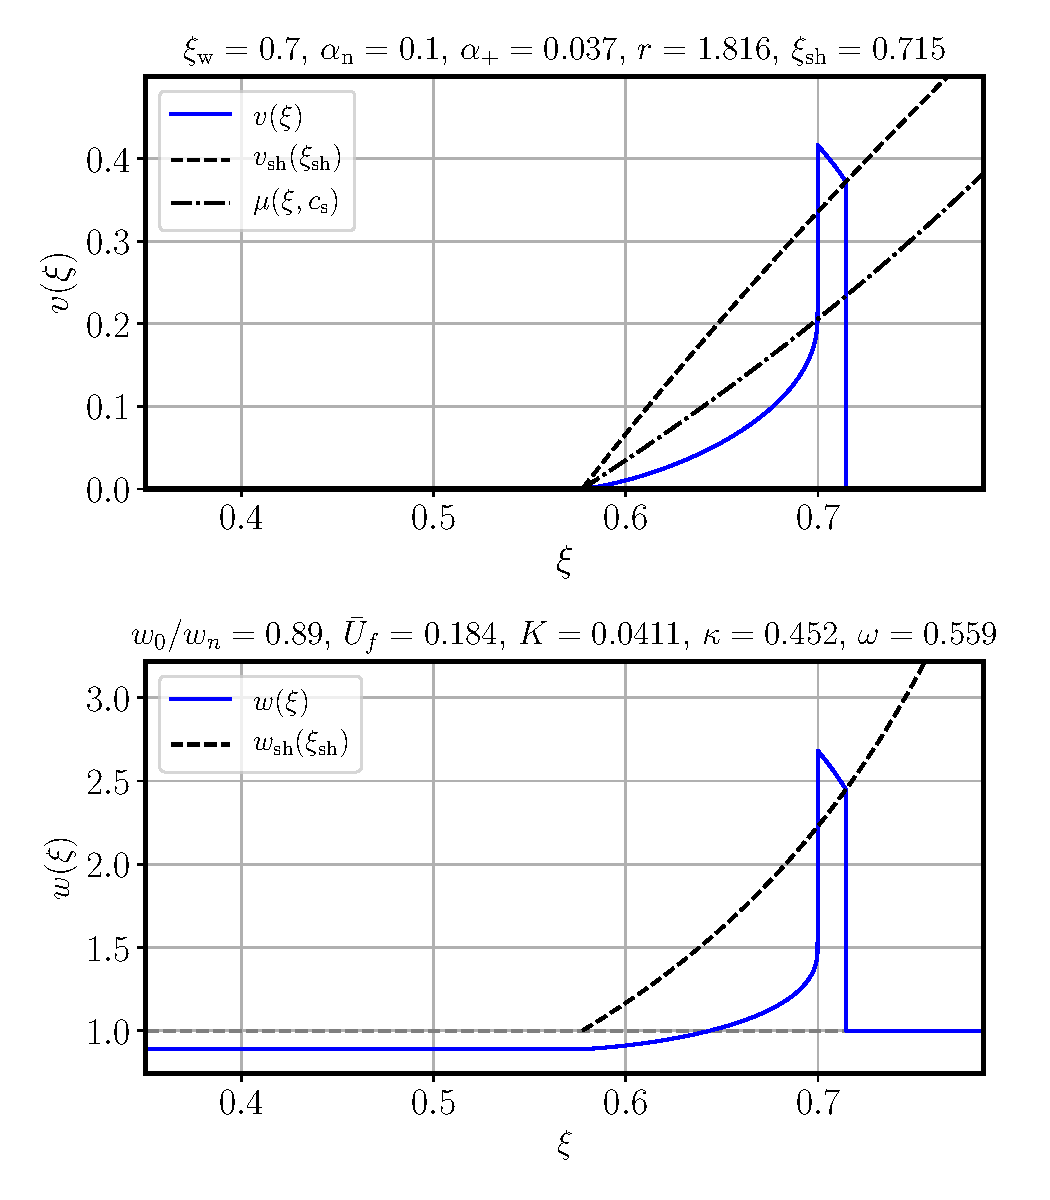
\includegraphics[width=0.2\textwidth]{../fig/shell_plot_vw_07_alphan_01_review.pdf}%
        TODO figure here
    \end{minipage}
\end{frame}

\begin{frame}
    \frametitle{Example result: entropy conservation}
    \begin{minipage}[t]{0.48\linewidth}
        \begin{itemize}
            \item 10 000 bubbles with varying $v_\text{wall}, \alpha_n$
            \item Top-left region ruled out by $\alpha_+ > \frac{1}{3}$
            \item Unphysical region (blue): decrease in total entropy
        \end{itemize}%
    \end{minipage}%
    \hfill%
    \begin{minipage}[t]{0.48\linewidth}%
        TODO figure here
    \end{minipage}
\end{frame}

\begin{frame}
    \frametitle{Gravitational wave production}
    \begin{itemize}
        \footnotesize
        \item Sound Shell Model (Hindmarsh, 2018)
        \item Velocity profile of a single bubble $v_\text{ip}(\xi)$ + sine transform \\ \textrightarrow \ velocity power spectrum
        \begin{align}
            \lambda(x) &= \frac{e(x) - \bar{e}}{\bar{w}} \\
            f(z) &= \frac{4 \pi}{z} \int_0^\infty d\xi v_\text{ip}(\xi) \sin(z\xi) \\
            l(z) &= \frac{4 \pi}{z} \int_0^\infty d\xi \lambda_\text{ip}(\xi) \xi \sin(z\xi) \\
            |A(z)|^2 &= \frac{1}{4} \left[ (f'(z))^2 + (c_s l(z))^2 \right]
        \end{align}
        \item Convolution with the nucleation rate function \\
            \textrightarrow Overall velocity power spectrum
        \item Convolution with a Green's function \textrightarrow \ GW power spectrum
        \begin{equation}
            \mathcal{P}_\text{gw} = \frac{1}{12 H^2} \frac{k^3}{2\pi^2} P_{\dot{h}}
        \end{equation}
    \end{itemize}
\end{frame}

\section{Conclusion}

\begin{frame}
    \frametitle{Summary}
    \begin{itemize}
        \item A phase transition converts energy from the scalar field to kinetic and thermal energy \textrightarrow Gravitational wave production
        \item The phase transition proceeds by bubble nucleation
        \item The hydrodynamics is based on energy-momentum conservation
        \item Solving a bubble starts with the equation of state
        \begin{itemize}
            \item Equation solving \& ODE integration \textrightarrow fluid velocity profile
            \item Sine transform \& convolutions \textrightarrow GW power spectrum
        \end{itemize}
        \item Sound shell model converts the velocity profile to GW power spectrum
        \item PTtools has been updated to deal with arbitrary equations of state
        \item PTtools will be published soon with support for arbitrary equations of state
    \end{itemize}
\end{frame}

\begin{frame}
    \frametitle{Sources}
    \begin{itemize}
        \scriptsize
        \item M. Hindmarsh, M. Lüben, J. Lumma, and M. Pauly, “Phase transitions in the early universe,” SciPost Phys. Lect. Notes, Feb. 2021, doi: 10.21468/SciPostPhysLectNotes.24.
        \item Hindmarsh, Mark, and Mulham Hijazi. “Gravitational Waves from First Order Cosmological Phase Transitions in the Sound Shell Model.” Journal of Cosmology and Astroparticle Physics 2019, Dec. 2019, doi: 10.1088/1475-7516/2019/12/062.
        \item Caprini et al. “Detecting Gravitational Waves from Cosmological Phase Transitions with LISA: An Update.” Journal of Cosmology and Astroparticle Physics 2020, Mar. 2020, doi: 10.1088/1475-7516/2020/03/024.
        \item Espinosa et al. “Energy Budget of Cosmological First-Order Phase Transitions.” Journal of Cosmology and Astroparticle Physics 2010, Jun. 2010, doi: 10.1088/1475-7516/2010/06/028.
        \item Giese et al., “Model-Independent Energy Budget for LISA.” Journal of Cosmology and Astroparticle Physics, Jan. 2021, doi: 10.1088/1475-7516/2021/01/072.
        \item Borsanyi, Sz, Z. Fodor, K. H. Kampert, S. D. Katz, T. Kawanai, T. G. Kovacs, S. W. Mages, et al. “Lattice QCD for Cosmology.”, Jun. 2016, ArXiv: 1606.07494
    \end{itemize}
\end{frame}

\begin{frame}
    % \frametitle{Thank you!}
    Thank you!
\end{frame}

\section{Extra slides}

% Extra backup slides
\begin{frame}
    \frametitle{Speedup example with Numba}
    \begin{itemize}
        \item Add JIT decorator
        \item Replace unsupported features with simpler code or split the unsupported parts to another function
        \item (Restructure the function to make the possible parallelism explicit)
    \end{itemize}
    {
        \footnotesize
        \lstset{escapeinside={<@}{@>}}
        \lstinputlisting[language=Python]{sin_transform_core.py}
    }
\end{frame}
